\documentclass{article}

\title{Reading08: Document Tools}
\date{}
\author{Andrew Munch}

\usepackage[pdftex]{graphicx}
\usepackage{hyperref}
\usepackage[margin=1in]{geometry}

\begin{document}

\maketitle

%--------------------------------------

\section*{Overview}

For this experiment, I created \verb|three| scripts:

   1. \verb|roll_dice.sh:| This sript simulates random dice rolls using the shuf command.
   2. \verb|experiment.sh:| This script uses \verb|roll_dice.sh| to simulate 1000 dice rolls and then output that data in tab-separated format into \verb|results.dat.|
   3. \verb|histogram.plt:| This script uses the gnuplot program to create a histogram of the data in \verb|results.dat.|

%--------------------------------------

\section*{Rolling Dice}

First, I created a script \verb|roll_dice.sh| that uses the shuf command to simulate random dice rolls.  The user can specify how many {\it sides} they would like to choose from and the number of {\it rolls} they would like to have.

\begin{verbatim}
$ ./roll_dice.sh -h
usage: roll_dice.sh [-r ROLLS -s sides]

-r ROLLS Number of rolls of die (default: 10)
-s SIDES Number of sides on die (default: 6)
\end{verbatim}

%---------------------------------------

\section*{Experiment}

Second, I created a script called \verb|experiment.sh| wich calls \verb|roll_dice.sh| with 1000 rolls.  This output is filtered using awk to create a list of tab-separated values that is then sent to a file \verb|results.dat|

%---------------------------------------

\section*{Results}

Table 1 shows the results of running the experiment shell script:

\begin{table}[h!]
	\centering
	\begin{tabular}{r|l||c}
	Side & Counts\\
	\hline
	1 & 162\\
	2 & 183\\
	3 & 160\\
	4 & 172\\
	5 & 157\\
	6 & 166\\
	\end{tabular}
	\caption{Dice Rolling Results}
	\label{tbl:rolls}
\end{table}

Figure 1 is a histogram plot of these results:

\begin{figure}[h!]
\centering
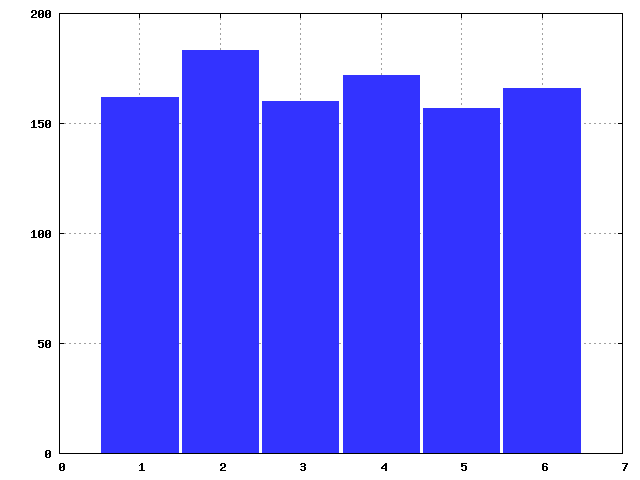
\includegraphics[width=5in]{results.png}
\caption{Dice Rolling Results}
\label{fig:rolls}
\end{figure}
